\srsfuncion{Consultar ficha empleado}
	Esta función debe mostrar al usuario la lista de empleados de la compañía, permitiendo buscar y filtrar resultados, así como información detallada de cada empleado en particular.
		
	\begin{enumerate}
		\item \textit{Prioridad}: alta.
		\item \textit{Entradas}
			\begin{enumerate}
				\item La lista de empleados se mostrará ordenada por defecto sugún nombres en orden alfabético, pero podrá ordenarse según: apellidos, NIF, fecha de nacimiento, tiempo trabajado en la empresa y departamento (Personal administrativo, Mecánico, Directivo, Personal de seguridad, Auxiliar de Vuelo y Piloto).							
			\end{enumerate}
		\item \textit{Flujo de operaciones}
			\begin{enumerate}
				\item Se muestra por pantalla una tabla con la lista de empleados ordenada por nombres en orden alfabético. Se da la opción al usuario de ordenarla siguiendo los criterios mencionados anteriormente.
				\item Para cada empleado que seleccione el usuario, habrá un botón \verb|Ver detalles...|, que permite acceder a la información detallada de dicho empleado.
			\end{enumerate}
		\item \textit{Respuesta a situaciones no previstas}
			\begin{enumerate}
				\item Si no se puede acceder a la base de datos de empleados: se muestra por pantalla un mensaje de error indicando el error producido y se vuelve a la página principal del sistema.
				\item Si no se ha podido ordenar en el orden deseado: mostrar la información desordenada y mostrar por pantalla un mensaje indicando que no se ha podido ordenar.
				\item Si no se puede acceder a la información detallada del empleado: mostrar un mensaje por pantalla informando al usuario del error y volver a la pantalla anterior.
			\end{enumerate}
	\end{enumerate}
	\begin{figure}[ht]\centering
	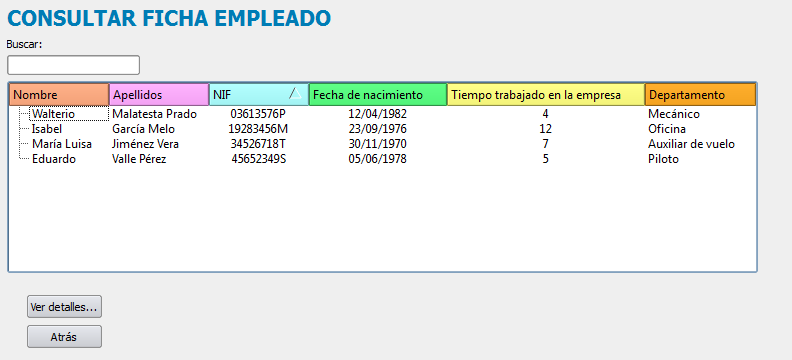
\includegraphics[scale=.6]{imagenes/consultarFichaEmpleadoImagen.png}
	\caption{Pantalla aproximada de la ficha de un empleado}
\end{figure}
								
